% 2009 年湖南卷文科第 18 题：正三棱柱 ABC-A1B1C1 及点 D、E。
% 来源 PDF：普通高考/2009/2009湖南文.pdf，SHA-256 db41a34b5d57a8db3f2ee49872e3dbc1e290c2e7390fc96cf4e084b5a679e3eb。
% 原页：第 1 页（A3 三栏）第 3 栏下部，书页码 529。
% 重绘依据：按原页斜视位置重绘，正三棱柱底面边长 AB=4、侧棱 AA1=√7（图上只按示意比例）。
%   可见：A1A、AB、BB1、A1B1、A1C1、C1B1 为实线；被柱体遮挡的 AC、CC1、CB 为虚线。
%   D 为 BC 中点、E 在 AC 上；辅助线 A1D、A1E、AD、AE、DE 均按原页画虚线。
%   投影取 (x,y,z) -> (x+0.20y, z+0.48y)，与原件 C 略偏于 AB 中点的斜视位置一致。
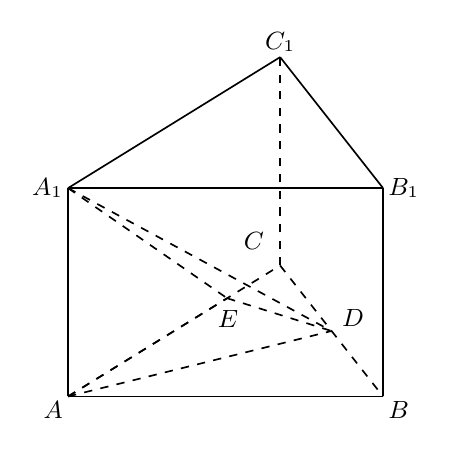
\begin{tikzpicture}[semithick, every node/.style={inner sep=1.6pt, font=\small}]
  % 底面 A(0,0,0)、B(4,0,0)、C(2,2√3,0)，高 √7
  \coordinate (A)  at (0.000,0.000);
  \coordinate (B)  at (4.000,0.000);
  \coordinate (C)  at (2.693,1.663);
  \coordinate (A1) at (0.000,2.646);
  \coordinate (B1) at (4.000,2.646);
  \coordinate (C1) at (2.693,4.309);
  % D 为 BC 中点；E 在 AC 上，AE:EC=3:1（由 DE⊥A1E 定出）
  \coordinate (D)  at (3.346,0.831);
  \coordinate (E)  at (2.020,1.247);

  % 可见棱
  \draw (A1) -- (A);
  \draw (A) -- (B);
  \draw (B) -- (B1);
  \draw (A1) -- (B1);
  \draw (A1) -- (C1);
  \draw (C1) -- (B1);

  % 被遮挡的棱
  \draw[dashed] (A) -- (C);
  \draw[dashed] (C) -- (C1);
  \draw[dashed] (C) -- (B);

  % 辅助线
  \draw[dashed] (A1) -- (D);
  \draw[dashed] (A1) -- (E);
  \draw[dashed] (A) -- (D);
  \draw[dashed] (A) -- (E);
  \draw[dashed] (E) -- (D);

  % 标注
  \node[left] at (A1) {$A_1$};
  \node[right] at (B1) {$B_1$};
  \node[above] at (C1) {$C_1$};
  \node[below left] at (A) {$A$};
  \node[below right] at (B) {$B$};
  \node at (2.360,1.980) {$C$};
  \node at (3.620,1.000) {$D$};
  \node at (2.030,0.980) {$E$};
\end{tikzpicture}
